\newpage
\subsection{Query-Answering Module}
\label{sec:QAModule}
Query-Answering Module offers users to create simple fuzzy queries or complex fuzzy queries by choosing negations, quantifications and fuzzy concepts which are defined in Configuration Modules. 
% Theoretical definition of Fuzzy Query
% Explain the functionality of Query-Answering Module
% How to use Interface
\subsubsection{Fuzzy Query}
In RFuzzy Framework, we define the fuzzy query as a pair $<A,v>$, where $A \in TB_{\Pi,\Sigma,V}$ and $v$ is either a ``new'' variable that represents the initially unknown truth value of $A$ or it is a concrete value $v \in [0,1]$ that is asked to be the truth value of $A$. We extend this simple query into complex one.

\begin{defin} \textbf{(Complex fuzzy query).}
\label{def:ComplexFuzzyQuery}
\[Answer(\vec{t},v) \stackrel{c,F_c}{\longleftarrow} F(p_1(\vec{t_1},v_1),...,p_m(\vec{t_m},v_m))\]
where $p_i$s are predicates in RFuzzy program $P$, $Answer$ is a predicate which never appears in program $P$, $v_i$ and $v$ could be unknown truth value for their associated atoms or concrete value $v$ assigned to their atoms.

\end{defin}

By introducing quantifiers into RFuzzy framework, it could be used to enhance the expressivity of the query, which is defined as follow,

\begin{defin} \textbf{(Simple fuzzy query with negation and quantification). }
\label{def:SFQNegQuan}
\[< A,v >\]
where $A$ is an atom $q(x_1, \dots, x_n)$. $q$ is represented as a regular expression, 
\[q= (Negation|Quantification)^*Predicate\]
\end{defin}

\begin{defin} \textbf{(Complex fuzzy query with negation and quantification). }
\label{def:CFQNegQuan}
\[Answer(\vec{t},v) \stackrel{c,F_c}{\longleftarrow} F(q_1(\vec{t_1},v_1),...,q_m(\vec{t_m},v_m))\]
where $Answer$ is a predicate that never appears in program $P$, $q_i$ is represented as a regular expression, 
\[q_i = (Negation|Quantification)^*Predicate\]
\end{defin}

\begin{ex}
A set of negations is $N=\{not, seldom\}$, a set of quantifiers is $Q=\{very, extremely\}$, and a set of fuzzy concept is $C=\{beautiful, clear\}$. The simple query with negation and quantification can be represented as `` not very beautiful girls ?", ``seldom extremely clear statements ?" and so on. A Complex query with negation and quantification is generated by joining those simple query together with fuzzy rules. The simplest complex query could be `` not very beautiful and seldom extremely clear landscape ?", which is formalized in fuzzy logic as,
\begin{align*}
Answer(Landscape, V) {\longleftarrow} & \textbf{min} & not(very(beautiful(Landscape))),\\ 
&  & seldom(extremely(clear(Landscape))). \\
\end{align*}
\end{ex}

\subsubsection{How to use interface of Query-Answering Module}
\begin{figure}[htb]
\begin{center}
\leavevmode
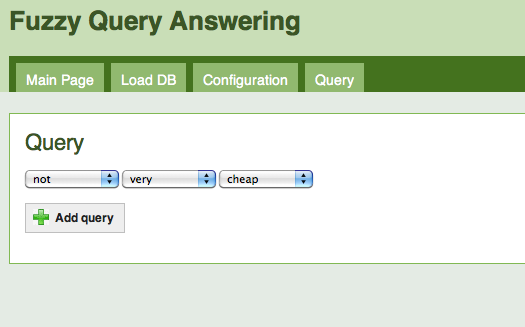
\includegraphics[scale=0.7]{Query.png}
\end{center}
\caption{Interface of Query-Answering Module}
\label{fig:QAMI}
\end{figure}
As shown in figure \ref{fig:QAMI}, users can choose negation, quantification, and fuzzy concept from  those three selection boxes. Users can add more queries by clicking button ``Add query", the previous query is listed on the right, and selection boxes are set to default empty ready for you to add more queries. By clicking button ``Query", the result will be generated and shown in a result page.